\documentclass[12pt,a4paper]{report}

% ==================== PACKAGES ====================
\usepackage[margin=1in]{geometry}
\usepackage{setspace}
\usepackage{fancyhdr}
\usepackage{titlesec}
\usepackage{tocloft}
\usepackage{booktabs}
\usepackage{enumitem}
\usepackage{hyperref}
\usepackage{graphicx}
\usepackage{xcolor}
\usepackage{caption}
\usepackage{subcaption}
\usepackage{longtable}
\usepackage{array}
\usepackage{multirow}
\usepackage{url}
\usepackage{xurl}  % better URL line breaking
\urlstyle{same}
\usepackage{listings}
\usepackage{float}
\usepackage{parskip}
\usepackage{microtype}
\usepackage{amsmath,amssymb}
\usepackage{tikz}
\usetikzlibrary{positioning,arrows.meta,shapes.geometric,calc}

% Hyperref setup
\hypersetup{
    colorlinks=true,
    linkcolor=blue!60!black,
    citecolor=blue!60!black,
    urlcolor=blue!70!black,
    pdftitle={Summer Internship Report - Learning Digital Design through phone-based Arduino Embedded Systems},
    pdfauthor={Ayaan Syed},
    pdfsubject={Internship Report, IIT Hyderabad},
}

% Page style
\setlength{\headheight}{14.5pt}
\pagestyle{fancy}
\fancyhf{}
\fancyhead[L]{\small\textit{EE Core Labs, IIT Hyderabad}}
\fancyhead[R]{\small\textit{Summer Internship Report}}
\fancyfoot[C]{\thepage}
\renewcommand{\headrulewidth}{0.4pt}
\renewcommand{\footrulewidth}{0.3pt}

% Section formatting
\titleformat{\chapter}[display]
{\normalfont\huge\bfseries\color{blue!40!black}}
{\chaptertitlename\ \thechapter}{20pt}{\Huge}
\titlespacing*{\chapter}{0pt}{-20pt}{30pt}

\titleformat{\section}
{\normalfont\Large\bfseries\color{blue!30!black}}
{\thesection}{1em}{}
\titleformat{\subsection}
{\normalfont\large\bfseries\color{blue!20!black}}
{\thesubsection}{1em}{}

% List spacing
\setlist[itemize]{leftmargin=*,itemsep=3pt,parsep=2pt}
\setlist[enumerate]{leftmargin=*,itemsep=3pt,parsep=2pt}

% Caption styling
\captionsetup{font=small,labelfont=bf}

% Code listing style (for GitHub links / code references)
\lstset{
    basicstyle=\ttfamily\small,
    breaklines=true,
    frame=single,
    backgroundcolor=\color{gray!5},
}

% ==================== DOCUMENT INFO ====================
\title{
    \vspace{-1.5cm}
    {\Large\textbf{Electrical Engineering Core Labs}}\\[0.3em]
    {\large Indian Institute of Technology Hyderabad (IIT Hyderabad)}\\[1.5em]
    {\Huge\textbf{SUMMER INTERNSHIP REPORT}}\\[0.8em]
    {\Large\textit{Learning Digital Design through\\phone-based Arduino Embedded Systems}}\\[1.5em]
    {\large May 23 -- July 15, 2026}
}
\author{
    Submitted by\\[0.5em]
    \textbf{Ayaan Syed}\\
    Jamia Millia Islamia, New Delhi\\[1.5em]
    Under the guidance of\\[0.5em]
    \textbf{Prof.\ G.V.V.}\\
    Department of Electrical Engineering,\\
    IIT Hyderabad
}
\date{}

% ==================== BEGIN DOCUMENT ====================
\begin{document}

\pagenumbering{roman}
\maketitle
\thispagestyle{empty}

\vspace{2cm}
\begin{center}
\begin{tabular}{@{}p{0.9\textwidth}@{}}
\hline
\vspace{0.3em}
\textbf{Declaration:} This report is a true account of the work carried out during the summer internship at the Electrical Engineering Core Labs, IIT Hyderabad, under the guidance of Prof.\ G.V.V. All sources and references have been duly acknowledged.\\[0.5em]
\hline
\end{tabular}
\end{center}

\clearpage
\tableofcontents
\clearpage
\pagenumbering{arabic}

% ============================================================
\chapter{Introduction}
\label{ch:intro}

This report presents a summary of the summer internship undertaken at the Electrical Engineering Core Labs, Indian Institute of Technology Hyderabad (IIT Hyderabad), from May 23, 2026 to July 15, 2026, under the guidance of Prof.\ G.V.V. The internship focused on Arduino programming and embedded systems, with an emphasis on understanding hardware-software interaction at multiple levels --- from high-level code down to assembly-level programming --- and on building a functional embedded project from the ground up.

Unlike a conventional Arduino IDE-based workflow using a laptop, this internship used an unconventional and highly hands-on approach: programming and uploading code to the Arduino using an Android phone via a USB OTG cable, using Termux as the development environment. This method required setting up a complete Linux-based command-line toolchain on a mobile device, giving deeper insight into how embedded toolchains work under the hood, rather than relying on the abstraction provided by desktop IDEs.

The internship progressed from foundational exercises with basic digital ICs to a substantial minor project --- the design, coding, and hardware assembly of a fully functional digital clock, including custom PCB-free assembly on a perfboard.

\section{About the Host Institute}
\label{sec:host}

The Indian Institute of Technology Hyderabad (IIT Hyderabad) is one of India's premier institutions for engineering education and research. Its Electrical Engineering Core Labs support undergraduate and intern learning through hands-on, lab-based courses that emphasize practical circuit design, embedded systems, and microcontroller programming alongside theoretical coursework. The Core Labs are equipped for both breadboard-level prototyping and permanent circuit assembly, making them well suited to project-based internships such as this one.

The internship was carried out under the direct guidance of Prof.\ G.V.V., whose instructional material --- including setup guides and package installation instructions published on GitHub --- formed the backbone of the toolchain used throughout the internship.

The internship spanned approximately eight weeks, structured broadly into three phases: an initial orientation and toolchain-setup phase, a foundational-exercises phase covering basic digital ICs, and a major-project phase centered on the design and construction of a standalone digital clock.

% ============================================================
\chapter{Objectives of the Internship}
\label{ch:objectives}

\begin{itemize}
    \item To gain hands-on experience with Arduino and embedded systems programming beyond the standard IDE workflow.
    \item To understand the three levels of embedded development: hardware design, software-level (compiled) code, and assembly-level code.
    \item To learn to set up and use a Linux-based mobile development environment (Termux) for compiling and uploading code to microcontrollers.
    \item To gain practical exposure to fundamental digital ICs such as the 7447 (BCD-to-7-segment decoder) and 7474 (D flip-flop / decade counter).
    \item To design, build, and test a digital clock circuit --- from breadboard prototyping to a soldered perfboard implementation.
    \item To learn bootloader burning and standalone microcontroller programming using an ATmega328P chip.
    \item To develop practical hardware debugging and soldering skills.
\end{itemize}

% ============================================================
\chapter{Internship Timeline}
\label{ch:timeline}

The internship ran for approximately eight weeks, from May 23 to July 15, 2026. The table below gives an approximate phase-wise breakdown of how the internship progressed, from initial environment setup through to the completed digital clock.

\begin{table}[H]
\centering
\caption{Phase-wise Internship Timeline}
\label{tab:timeline}
\begin{tabular}{@{}>{\bfseries}lp{10.8cm}@{}}
\toprule
Period & \textbf{Activities} \\
\midrule
Week 1 & Orientation; introduction to the lab, to Prof.\ G.V.V.'s workflow, and to the overall goals of the internship. \\
Week 2 & Setting up Termux and Linux on the phone and laptop; installing toolchain packages from GitHub instructions; first successful compile-and-upload cycle on the Arduino Uno. \\
Week 3 & Learning and practicing the three-step workflow (hardware, software-level code, assembly-level code) on simple I/O tasks. \\
Week 4 & Foundational tasks: seven-segment display interfacing, and working with the 7447-decoder IC. Also worked on \LaTeX\ documentation of a question paper using Neovim as the editor, including implementing a watermark and other key formatting features. \\
Week 5 & Foundational tasks continued: working with the 7474 D flip-flop and building decade counter circuits; a GATE problem was also implemented on the breadboard using Arduino; transition into planning the digital clock project. \\
Week 6 & Digital clock: breadboard prototyping and testing using the Arduino Uno. \\
Week 7 & Digital clock: bootloader burning and programming of standalone ATmega328P chips; standalone breadboard testing. \\
Week 8 & Digital clock: perfboard soldering, assembly, debugging, and final validation; wrap-up and report preparation. \\
\bottomrule
\end{tabular}
\end{table}

% ============================================================
\chapter{Tools, Software and Setup}
\label{ch:tools}

The internship made use of an unconventional but effective toolchain built entirely around a smartphone, in place of a traditional laptop-based Arduino IDE setup. The core components of this setup are summarized below.

\begin{table}[H]
\centering
\caption{Core Tools and Components}
\label{tab:tools}
\begin{tabular}{@{}>{\bfseries}p{3.6cm}p{10.5cm}@{}}
\toprule
Component & \textbf{Details} \\
\midrule
Microcontroller & Arduino Uno; standalone ATmega328P chips \\
Development Environment & Termux (Linux terminal emulator for Android) \\
Upload Interface & Arduino Droid (Android app, using ``Upload Precompiled'') \\
Connection & USB OTG cable (phone to Arduino Uno) \\
Operating System & Linux, installed both within Termux and on the lab laptop \\
Toolchain Packages & Installed via Termux using package installation instructions provided by Prof.\ G.V.V.\ through GitHub \\
Prototyping Hardware & Breadboard, perfboard, jumper wires, copper wire, soldering iron \\
ICs Used & 7447 (BCD-to-7-segment decoder), 7474 (D flip-flop / decade counter) \\
\bottomrule
\end{tabular}
\end{table}

Setting up Termux involved installing the Linux command-line environment on the phone and then downloading the required compiler and toolchain packages using setup instructions shared by Prof.\ G.V.V.\ on GitHub. This setup effectively turned the phone into a portable embedded development workstation, capable of writing, compiling, and flashing code directly to Arduino hardware without a laptop.

In parallel, a full Linux operating system was also installed on the lab laptop. Having both a phone-based (Termux) and a laptop-based Linux environment available meant that the same command-line toolchain --- compilers, assemblers, and AVR upload utilities --- could be used consistently across devices, reinforcing the idea that embedded development does not have to be tied to a specific IDE or operating system, but rather to a portable, script-driven toolchain.

This setup stood in deliberate contrast to the conventional Arduino IDE, which hides most of the compilation and upload process behind a single ``Upload'' button. By instead compiling code manually within Termux, saving the output to the Downloads folder, and uploading it through ArduinoDroid's ``Upload Precompiled'' option, each stage of the process --- compilation, file generation, and flashing --- had to be understood and executed as a distinct, visible step.

% ============================================================
\chapter{Methodology: The Three-Step Development Workflow}
\label{ch:methodology}

Every task during the internship, regardless of complexity, followed a consistent three-step workflow that mirrored the actual layers of embedded system development:

\begin{enumerate}
    \item \textbf{Hardware Design} --- Planning and building the physical circuit, including component selection and wiring on breadboard or perfboard.
    \item \textbf{Software-Level Code} --- Writing the logic in C/C++ within Termux, compiling it on-device, saving the compiled output to the phone's Downloads folder, and uploading it to the Arduino using Arduino Droid's ``Upload Precompiled'' feature.
    \item \textbf{Assembly-Level Code} --- Writing and compiling equivalent assembly code, generating the corresponding \texttt{.hex} file, saving it to Downloads, and uploading it via the same ``Upload Precompiled'' route in Arduino Droid.
\end{enumerate}

Working through both the software and assembly levels for the same hardware task reinforced a clear understanding of what happens between writing code and it actually running on a microcontroller --- including compilation, hex file generation, and how precompiled binaries are flashed onto hardware.

% ============================================================
\chapter{Foundational Tasks}
\label{ch:foundational}

Before progressing to the minor project, several foundational exercises were completed to build familiarity with the hardware-software-assembly workflow and with basic digital ICs.

\section{Seven-Segment Display}
\label{sec:sevenseg}

A basic seven-segment display was interfaced with the Arduino, driven at both the software and assembly level, to understand digit-pattern generation and I/O pin control. At the software level, this meant writing code that mapped each digit (0--9) to the correct combination of segment pins to switch on; at the assembly level, the same mapping had to be implemented through direct register and port manipulation, without the convenience of higher-level variables or functions. Comparing the two implementations for the exact same task made the relationship between high-level code and the underlying register operations much clearer.

\begin{itemize}
    \item Code: \url{https://github.com/gadepall/fwc-1/blob/main/ide/sevenseg/codes/sevenseg/sevenseg.ino}
\end{itemize}

\section{IC 7447 -- BCD to Seven-Segment Decoder}
\label{sec:7447}

The 7447-decoder IC was used to convert binary-coded decimal (BCD) input into the signals needed to drive a seven-segment display directly, reducing the number of Arduino pins required for display control. Rather than driving each of the seven display segments individually from the Arduino, only four BCD input lines needed to be controlled, with the 7447 handling the decoding logic in hardware. This task illustrated a recurring theme of the internship: how dedicated ICs can offload logic that would otherwise have to be implemented entirely in software.

\begin{itemize}
    \item Code: \url{https://github.com/gadepall/fwc-1/blob/main/ide/7447/codes/gvv_ard_7447/gvv_ard_7447.ino}
    \item Code (Increment/Decrement): \url{https://github.com/gadepall/digital-design/blob/main/ide/7447/codes/inc_dec/inc_dec.ino}
    \item Code (Input Increment/Decrement): \url{https://github.com/gadepall/fwc-1/blob/main/ide/7447/codes/ip_inc_dec/ip_inc_dec.ino}
\end{itemize}

\section{IC 7474 -- D Flip-Flop / Decade Counter}
\label{sec:7474}

The 7474 D flip-flop was used to build and study decade counter behaviour, forming a key building block later reused conceptually in the digital clock's timekeeping logic. We used two 7474 ICs, one 7447 and a 7-segment display. Since each 7474 contains two flip-flops, in total there are four flip-flops. Therefore the number of states is $\leq 16$; with the help of the coding logic, a counter of 10 states was realized. Understanding how flip-flops chain together to divide and count clock pulses was directly relevant to the digital clock project, where seconds, minutes, and hours all rely on the same underlying principle of counting and rolling over at fixed intervals.

\begin{figure}[H]
\centering
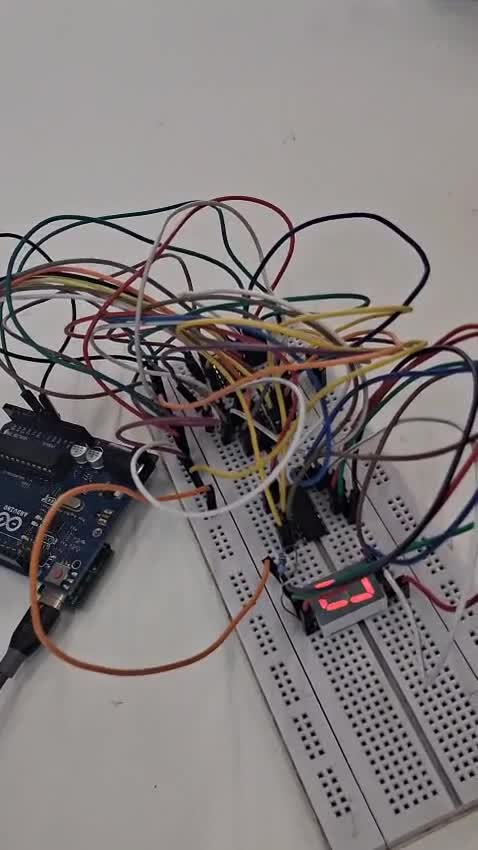
\includegraphics[width=0.55\textwidth]{image1.jpg}
\caption{Frame from the video demonstration of the 7474-decade counter circuit in operation.}
\label{fig:7474}
\end{figure}

% ============================================================
\chapter{Gate Problem: GATE EE 2019, Q44}
\label{ch:gate}

As an extension of the work on basic digital ICs, a GATE-level digital logic problem (GATE EE 2019, Question 44) was also implemented and verified on the breadboard using the Arduino, as part of the Week 5 activities. The question, along with the circuit to be simplified, is reproduced below.

\begin{figure}[H]
\centering
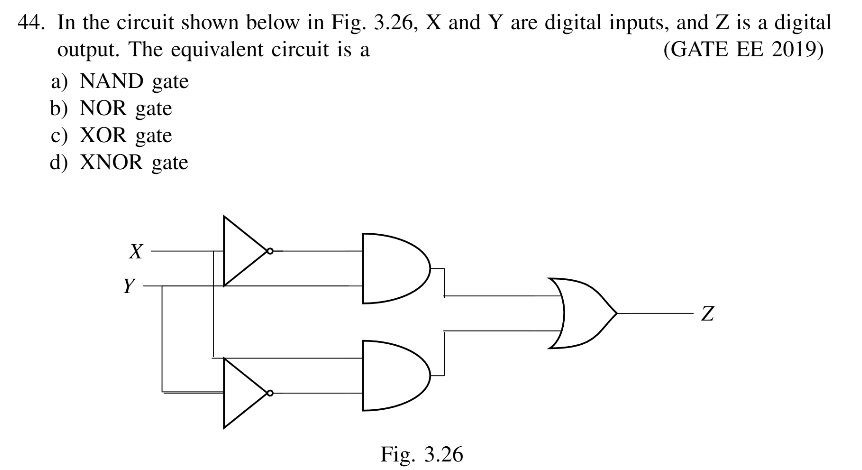
\includegraphics[width=0.92\textwidth]{image2.png}
\caption{GATE EE 2019, Q44 --- equivalent logic circuit for digital inputs $X$, $Y$ and digital output $Z$.}
\label{fig:gateq44}
\end{figure}

In the circuit, $X$ and $Y$ are first passed through NOT gates and combined with the original signals using two AND gates, whose outputs are then combined using an OR gate to produce $Z$. Working through the Boolean expression for this arrangement shows that it reduces to the XOR function of $X$ and $Y$, making the correct answer option (c) XOR gate. Rebuilding this circuit on the breadboard with discrete NOT, AND, and OR gate ICs, and verifying its truth table against an Arduino-driven XOR gate, confirmed this equivalence in hardware rather than only algebraically.

\begin{itemize}
    \item Code: \url{https://github.com/ayaansyed8/GATE-Q/blob/main/Gate}
\end{itemize}

% ============================================================
\chapter{LaTeX Documentation of Question Paper}
\label{ch:latex}

In Week 4, a GATE-style Computer Science and IT question paper was typeset in \LaTeX, edited entirely in Neovim and compiled with \texttt{pdflatex}. The document uses a custom header/footer with an institute logo (\texttt{fancyhdr}), a faint page watermark (\texttt{eso-pic}, \texttt{transparent}), custom \texttt{\textbackslash question} and \texttt{\textbackslash mcqtable} macros for consistent formatting across all 65 questions, structured tables (\texttt{booktabs}, \texttt{tabularx}), and \texttt{tikz}-drawn figures.

\begin{itemize}
    \item Source: \texttt{Question\_Paper\_LaTeX\_Source.tex}
\end{itemize}

% ============================================================
\chapter{Minor Project: Digital Clock}
\label{ch:clock}

The major portion of the internship was dedicated to designing, building, and testing a fully functional digital clock --- from an Arduino-driven breadboard prototype to a final, independently powered, soldered circuit built around a standalone ATmega328P chip. This project brought together every concept covered in the foundational tasks: digital display driving, counter logic, and the three-step hardware/software/assembly workflow, applied at a larger and more integrated scale.

\section{Design Approach}
\label{sec:design}

The clock was approached in clearly separated stages rather than being built end-to-end in one attempt. Each stage was fully validated before moving to the next: circuit logic on the breadboard first, then standalone chip behaviour, and only then permanent soldered assembly. This staged approach meant that if something failed later on, the number of possible causes to check was much smaller, since the earlier stages had already been confirmed working. This sequencing was itself one of the more valuable practical lessons of the project.

\section{Breadboard Prototype}
\label{sec:breadboard}

The digital clock circuit was first built and tested on a breadboard, with the Arduino Uno used directly to flash and run the clock logic. Building on the breadboard first, rather than soldering immediately, allowed the wiring and component placement to be adjusted freely while the timekeeping logic was being written and debugged. This stage validated the overall circuit design and timing logic before committing to a standalone, soldered implementation, and served as the working reference circuit for every later stage of the project.

\begin{figure}[H]
\centering
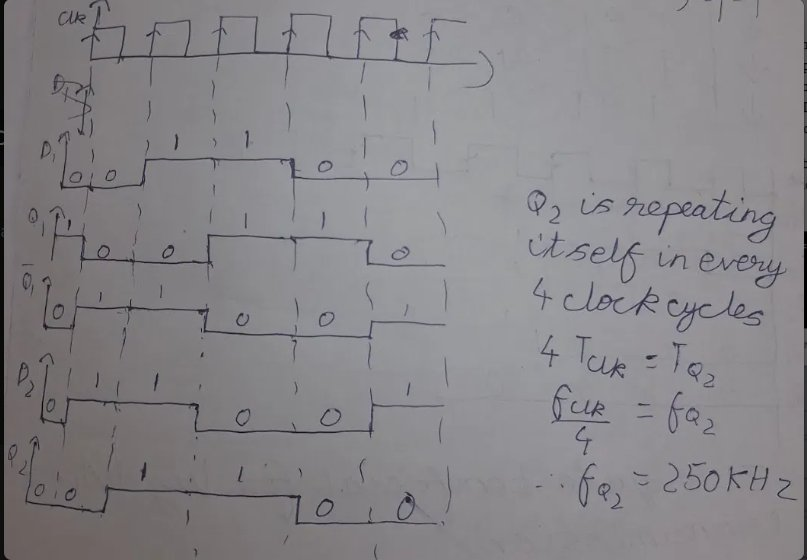
\includegraphics[width=0.85\textwidth]{image6.jpg}
\caption{Digital clock breadboard prototype with seven-segment displays driven by the Arduino Uno.}
\label{fig:breadboard}
\end{figure}

\section{Bootloader Burning and Standalone ATmega328P Programming}
\label{sec:bootloader}

To move beyond the Arduino Uno board itself, individual ATmega328P chips were programmed to run standalone --- that is, without being mounted on an Arduino Uno board at all. This involved burning the bootloader onto each bare chip, a process that reconfigures the chip's fuse settings so that it can subsequently accept and run uploaded programs on its own, exactly as an Arduino Uno's onboard microcontroller does out of the box.

Once bootloaded, the Arduino Uno itself was repurposed as an in-system programmer (ISP), used to upload the compiled clock code directly onto each individual standalone ATmega328P chip. This step required care, since an incorrect fuse configuration or a failed upload would leave the chip unresponsive and require the bootloading process to be repeated from scratch.

\section{Standalone Testing}
\label{sec:standalone}

Each programmed standalone ATmega328P chip was then tested on the breadboard circuit, independent of the Arduino Uno board, to confirm that the clock logic ran correctly on the bare chip before moving to permanent assembly. This step was an important checkpoint: any issue caught here on the breadboard was far easier and quicker to fix than the same issue discovered later, after the circuit had already been soldered onto the perfboard.

\section{Perfboard Assembly and Soldering}
\label{sec:perfboard}

Once the standalone circuit was validated, the design was transferred to a perfboard for a permanent build. This involved soldering all components --- the standalone ATmega328P, supporting passive components, and the clock display --- in place, and manually routing connections using copper wire in place of the Arduino Uno's internal traces and the breadboard's reconfigurable strips.

This stage was significantly more hands-on and unforgiving than breadboard prototyping. On a breadboard, a wrong connection can be pulled out and replaced in seconds; on a soldered perfboard, correcting a mistake means desoldering, which risks damaging components or lifting copper pads. As a result, this phase demanded far greater attention to planning the physical layout before soldering began, and it was also where most of the debugging time during the internship was spent.

\begin{figure}[H]
\centering
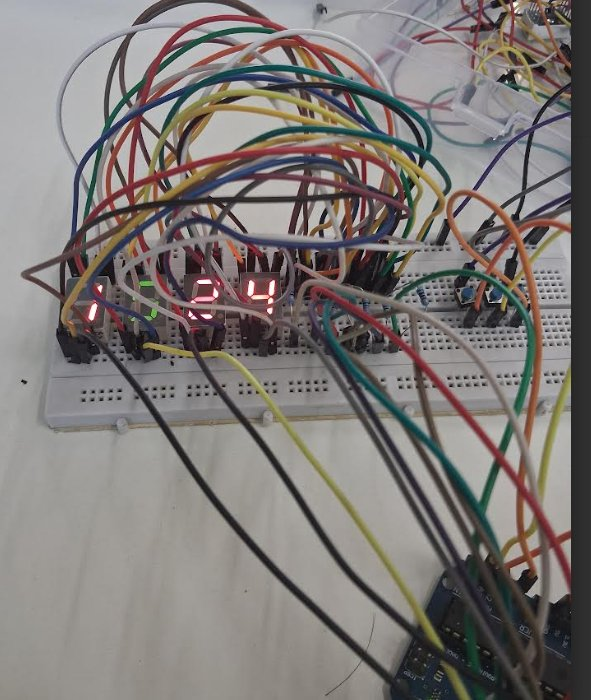
\includegraphics[width=0.85\textwidth]{image7.jpg}
\caption{Soldered perfboard assembly of the digital clock circuit, with copper-wire connections.}
\label{fig:perfboard}
\end{figure}

\section{Final Testing and Validation}
\label{sec:final}

After assembly, the soldered digital clock was powered and tested independently of the breadboard prototype and the Arduino Uno, confirming that the standalone board --- chip, bootloader, uploaded code, and physical wiring --- functioned correctly as a complete, self-contained unit.

% ============================================================
\chapter{Digital Electronics}
\label{ch:digitalelec}

Alongside the hardware and documentation work, time was also set aside to strengthen the underlying fundamentals of digital electronics, which proved essential to the rest of the internship. This was done by working through GATE-level questions provided in Prof.\ G.V.V.'s reference material, while building up the core concepts from Morris Mano's \textit{Digital Design} --- connecting the theory of Boolean simplification, Karnaugh maps, and prime implicants directly to the circuits being built on the breadboard.

One representative example is a four-variable minimization problem, solved by constructing the Karnaugh map, identifying the prime implicants and essential prime implicants, and reading off the minimum SOP and POS expressions.

\begin{figure}[H]
\centering
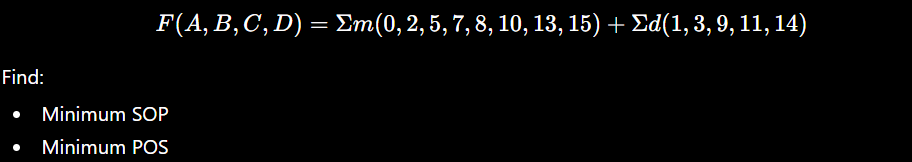
\includegraphics[width=0.92\textwidth]{image3.png}
\caption{GATE-style Boolean minimization question --- find the minimum SOP and minimum POS.}
\label{fig:kmapq}
\end{figure}

\begin{figure}[H]
\centering
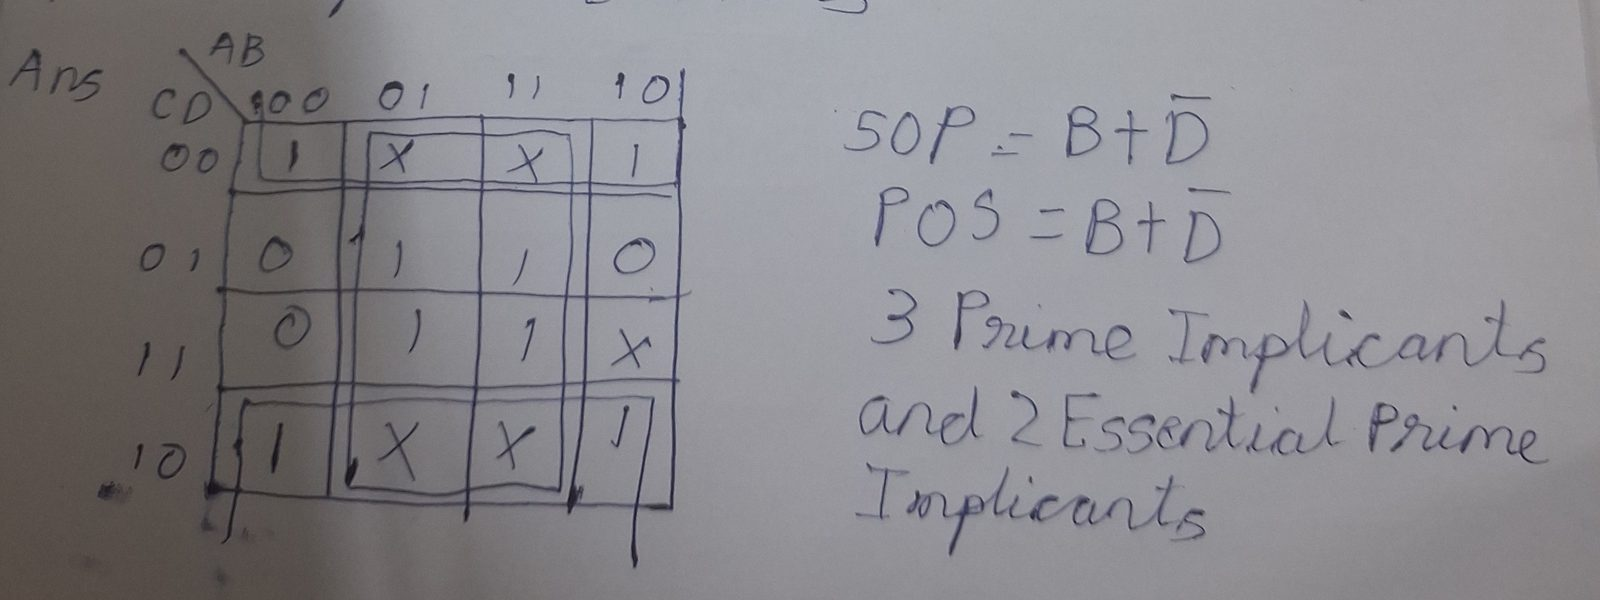
\includegraphics[width=0.95\textwidth]{image4.jpg}
\caption{Worked solution --- Karnaugh map, prime implicants, and minimum SOP/POS expressions.}
\label{fig:kmapsol}
\end{figure}

A second representative example involves a sequential circuit built from two D flip-flops, where the task is to determine the output frequency of $Q_2$ given an initial state and a known clock frequency. This was solved by tracing the timing diagram of each signal cycle by cycle to identify the repeating pattern of $Q_2$ relative to the clock.

\begin{figure}[H]
\centering
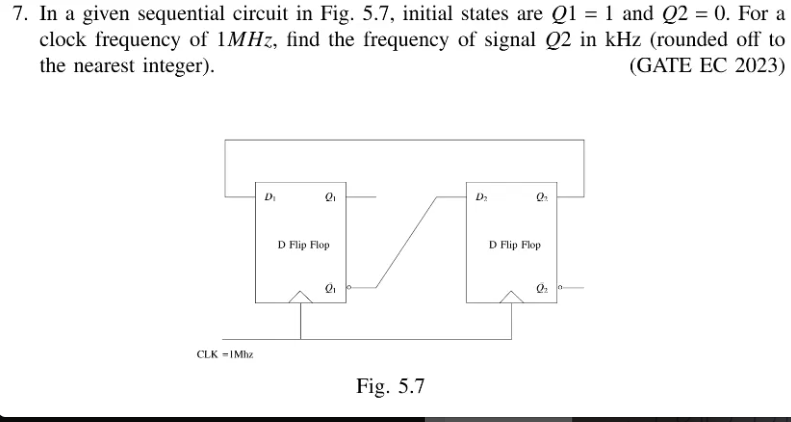
\includegraphics[width=0.90\textwidth]{image5.png}
\caption{GATE EC 2023 --- sequential circuit with two D flip-flops; find the frequency of $Q_2$.}
\label{fig:seqq}
\end{figure}

\begin{figure}[H]
\centering
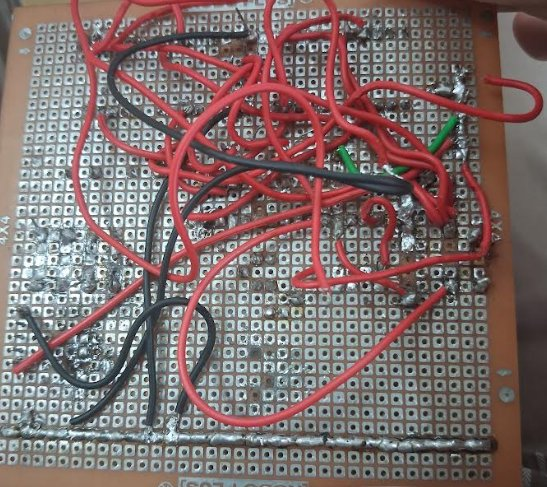
\includegraphics[width=0.75\textwidth]{image8.jpg}
\caption{Worked solution --- timing diagram showing $Q_2$ repeating every 4 clock cycles, giving $f_{Q_2} = 250\,\mathrm{kHz}$.}
\label{fig:seqsol}
\end{figure}

% ============================================================
\chapter{Challenges Faced}
\label{ch:challenges}

Working with real hardware, rather than software alone, meant that several of the biggest challenges during the internship were physical and diagnostic in nature rather than purely programming-related.

\section{Unconventional Development Workflow}
\label{sec:workflowchal}

Adapting to a phone-based development workflow using Termux and Arduino Droid, instead of a standard laptop IDE, required extra discipline at each of the three workflow steps. There was no single ``Upload'' button to fall back on --- every compile, file save, and precompiled upload had to be performed correctly and in the right order, and a mistake at any one step (for example, uploading an outdated file from Downloads) could produce confusing results that looked like a hardware fault.

\section{Short Circuits and Component Damage}
\label{sec:shorts}

Short-circuiting components --- including LEDs --- occurred at multiple points during breadboard and perfboard work, particularly when wiring density increased in the more complex clock circuit. These incidents occasionally damaged parts outright, requiring them to be replaced and the affected section of the circuit rebuilt and retested from scratch.

\section{Diagnosing Faults After Soldering}
\label{sec:diagnose}

By far the most time-consuming challenge was diagnosing faulty hardware connections after soldering on the perfboard. Unlike a breadboard, where a suspect connection can simply be unplugged and tested, a soldered joint has to be visually inspected, probed with a multimeter, or in some cases desoldered entirely to confirm whether it is the source of a fault. Narrowing down which specific component or connection was not working --- versus a fault elsewhere in the circuit or in the uploaded code --- often took considerably longer than the soldering itself.

\section{Bootloader and Fuse Configuration}
\label{sec:fuse}

Ensuring correct fuse settings and successful bootloader burns on standalone ATmega328P chips required careful attention, since a single misconfigured step would leave the chip unable to run any uploaded code at all, with little direct feedback about what had gone wrong. This meant that failures at this stage often had to be diagnosed by re-checking the entire bootloading procedure rather than by examining the chip itself.

% ============================================================
\chapter{Learning Outcomes and Reflection}
\label{ch:outcomes}

Beyond the specific technical skills listed below, the internship reinforced a broader lesson about embedded systems development: that the gap between code and physical hardware is where most real engineering challenges live. Writing correct code was often the easier half of any given task; making that code run reliably on physical, sometimes imperfect, hand-soldered hardware required patience, systematic debugging, and a willingness to re-check assumptions at every layer, from fuse bits to cold solder joints.

Working through the three-step workflow --- hardware, software-level code, and assembly-level code --- for the same tasks also gave a much more concrete understanding of what a conventional Arduino IDE normally does automatically. Having to compile, generate hex files, and upload precompiled binaries manually made the underlying embedded toolchain visible rather than hidden, which is knowledge that carries over to working with other microcontroller platforms in the future.

% ============================================================
\chapter{Skills Gained}
\label{ch:skills}

\begin{itemize}
    \item Embedded C/C++ programming and assembly-level programming for AVR microcontrollers.
    \item Practical understanding of the compilation and flashing pipeline: source code $\rightarrow$ compiled binary/hex file $\rightarrow$ hardware upload.
    \item Command-line proficiency using Linux and Termux for embedded development.
    \item Working knowledge of digital ICs (7447, 7474) and their role in display and counter circuits.
    \item Bootloader burning and standalone microcontroller programming using Arduino as an ISP.
    \item Circuit prototyping on breadboards and permanent circuit assembly through soldering on perfboards.
    \item Hardware debugging --- systematically isolating faulty components and connections in both prototype and soldered circuits.
    \item Learnt several key concepts of Digital Electronics related to Latches, Flip Flops (SR, JK, D, T).
    \item Learnt the basics about Finite State Machine (FSM).
    \item Learnt to draw the timing diagrams of waveforms of digital signals in a circuit, cycle by cycle.
\end{itemize}

% ============================================================
\chapter{Conclusion}
\label{ch:conclusion}

This internship at the Electrical Engineering Core Labs, IIT Hyderabad, provided substantial hands-on exposure to embedded systems development, from low-level assembly programming to physical circuit assembly. Working through the complete pipeline --- hardware design, software-level coding, and assembly-level coding --- on real hardware, using an unconventional phone-based toolchain, offered a far deeper understanding of how embedded systems function than a typical IDE-based workflow would have. The culmination of this experience in an independently built, soldered digital clock, built around a standalone, bootloader-programmed ATmega328P chip, demonstrated the practical application of every concept covered during the internship. The debugging challenges encountered along the way, particularly during the soldering and testing phases, strengthened problem-solving skills that are broadly applicable to embedded hardware work.

I am grateful to Prof.\ G.V.V.\ and the Electrical Engineering Core Labs at IIT Hyderabad for the opportunity, guidance, and resources provided throughout this internship.

% ============================================================
\appendix

\chapter{Glossary of Key Terms}
\label{app:glossary}

The following terms, specific to the tools and workflow used during this internship, are summarized here for reference.

\begin{description}[style=nextline,leftmargin=3.5cm,font=\bfseries]
    \item[Termux] A terminal emulator and Linux environment app for Android, used here to write and compile embedded code directly on a smartphone.
    \item[ArduinoDroid] An Android application that can upload code to Arduino boards; used specifically in ``Upload Precompiled'' mode to flash binaries and hex files compiled in Termux.
    \item[USB OTG] USB On-The-Go --- a cable/adapter standard that allows a smartphone to act as a USB host, enabling a direct wired connection between the phone and the Arduino Uno.
    \item[Bootloader] A small pre-installed program on a microcontroller that allows new code to be uploaded to it without a separate hardware programmer; ``burning'' a bootloader installs this program and sets the associated fuse bits.
    \item[Fuse Bits] Configuration bits on an AVR microcontroller (such as the ATmega328P) that determine low-level hardware behavior, including clock source and bootloader presence.
    \item[ISP (In-System Programmer)] A method of programming a microcontroller directly, without going through its bootloader; here, an Arduino Uno was configured to act as an ISP for standalone ATmega328P chips.
    \item[ATmega328P] The AVR microcontroller chip used on the Arduino Uno board; in this internship, standalone versions of this chip were bootloaded and programmed independently of the Uno board.
    \item[Hex File] A file format (Intel HEX) containing compiled machine code in a form that can be uploaded directly onto a microcontroller's program memory.
    \item[Perfboard] A rigid board with a grid of pre-drilled holes and copper pads, used for permanently soldering and wiring together electronic components, as opposed to a reusable breadboard.
\end{description}

\chapter{References and Resources}
\label{app:refs}

\begin{itemize}
    \item Setup and package installation instructions provided by Prof.\ G.V.V., Department of Electrical Engineering, IIT Hyderabad (shared via GitHub).
    \item Termux documentation, for Linux environment setup and package management on Android.
    \item ArduinoDroid application documentation, for the ``Upload Precompiled'' workflow.
    \item Datasheets for the 7447 BCD-to-seven-segment decoder and 7474 dual D-type flip-flop ICs.
    \item ATmega328P microcontroller datasheet, for fuse bit configuration and bootloader specifications.
    \item Morris Mano, \textit{Digital Design}.
\end{itemize}

\end{document}
